% !TeX root = ../my-thesis.tex
\chapter{Energieeffizientes Multithreading}

\section{Darstellung der Messwerte}

In diesem Kapitel werden die Ergebnisse der Messungen für die Untersuchung des Zusammenhangs zwischen Multithreading und der Energieeffizienz vorgestellt. Für diese Untersuchung wurden insgesamt 16 Messungen der Ausführung des Base64-Encoders mit steigender Anzahl von Threads unternommen. Die letzte Messung wurde mit 16 Threads durchgeführt. Dies entspricht der doppelten Anzahl an vorhanden physischen Rechenkernen des verwendeten Gerätes. Um den Zeitrahmen dieser Untersuchung nicht zu sprengen, wurden keine Messungen mit einer noch größeren Anzahl von Threads durchgeführt. An dieser Stelle sei gesagt, dass trotz der Begrenzung auf 16 Threads eine klare Tendenz zu erkennen ist, welche weitere Messungen überflüssig machen könnte.

In \autoref{tab:Base64Laufzeit} sind zunächst die ermittelten Laufzeiten der Ausführungen mit steigender Anzahl von Threads zu sehen. Es ist erkennbar, dass bis zu der Marke von 11 Threads ein stetiger Zuwachs an Ausführungsgeschwindigkeit zu erkennen ist, da die Laufzeit bis zu diesem Punkt konstant abnimmt. Zwar ist die Ausführung ab 12 Threads immer noch performanter als ursprünglich, verliert jedoch mit wachsender Anzahl an Threads allmählich an Geschwindigkeit.

% Table generated by Excel2LaTeX from sheet 'Tabelle1'
\begin{table}[htbp]
  \centering
  \caption{Laufzeit in Abh\"angigkeit von der Thread Anzahl}
    \begin{tabular}{rrrr}
    \toprule
    \multicolumn{1}{c}{Threads} & \multicolumn{1}{c}{t in ms} & \multicolumn{1}{l}{Speedup} & \multicolumn{1}{l}{Effizienz} \\
    \midrule
    1     & 994358 & 1,000 & 1,000 \\
    \midrule
    2     & 631836 & 1,574 & 0,787 \\
    \midrule
    3     & 507871 & 1,958 & 0,653 \\
    \midrule
    4     & 441615 & 2,252 & 0,563 \\
    \midrule
    5     & 416036 & 2,390 & 0,478 \\
    \midrule
    6     & 387519 & 2,566 & 0,428 \\
    \midrule
    7     & 369424 & 2,692 & 0,385 \\
    \midrule
    8     & 364560 & 2,728 & 0,341 \\
    \midrule
    9     & 364637 & 2,727 & 0,303 \\
    \midrule
    10    & 355893 & 2,794 & 0,279 \\
    \midrule
    11    & 355677 & 2,796 & 0,254 \\
    \midrule
    12    & 364313 & 2,729 & 0,227 \\
    \midrule
    13    & 363055 & 2,739 & 0,211 \\
    \midrule
    14    & 377380 & 2,635 & 0,188 \\
    \midrule
    15    & 383928 & 2,590 & 0,173 \\
    \midrule
    16    & 395553 & 2,514 & 0,157 \\
    \bottomrule
    \end{tabular}%
  \label{tab:Base64Laufzeit}%
\end{table}%


In \autoref{fig:Base64LeistungPic} ist ein Diagramm dieser Entwicklung zu sehen. Da im Testgerät acht physische Rechenkerne verbaut sind kan das das Gerät nur bis zu acht Threads wirklich parallel bearbeiten. Ab der Marke von neun Threads, ist die \ac{cpu} gezwungen ständig zwischen den Threads hin und her zu wechseln. Diese Art der Ausführung ist zwar noch nebenläufig aber nicht vollständig parallel. Bei jedem Kontextwechsel, muss der Status der Ausführung des aktuellen Threads gespeichert werden sodass die \ac{cpu} später an der richtigen Stelle mit der Berechnung fortfahren kann. Das Speichern und Laden der Register- und Prozessinformationen bei solch einem Kontextwechsel fordert Rechenaufwand und Zeit \cite[2]{MultiThreadingThesis}. Mit steigender Anzahl von Threads verstärkt sich dieser Effekt. Nun könnte die Annahme getroffen werden, dass aus diesem Grund die optimale Thread-Anzahl gleich der Anzahl an physischen Threads ist. Dies würde im Fall des hier verwendeten Gerätes bedeuten, dass acht Threads die schnellste Laufzeit erreichen müssten. Es ist jedoch zu erkennen, dass die Ausführung mit 11 Threads das beste Ergebnis liefert. Hierbei wurde mit 355677 \ac{ms} 63,3 \% weniger Laufzeit benötigt als mit einem Thread. Mit acht Threads hingegen sind es mit 364560 \ac{ms} nur 63,3 \% weniger. Eine weitere Auffälligkeit ist der massive Geschwindigkeitszuwachs bei dem Übergang von einem Thread zu zwei Threads. Der Speedup $S_{p}(2)$ nach \autoref{eq:Amdahlsche Gesetz} beträgt 1,57 und die daraus ermittelte Laufzeiteffizienz für zwei Threads $E_{ p }(2)$ nach \autoref{eq:Effizienz} beträgt 0,79 \todo{speedup und Effizienz in tagbelle ergänzen }. Statt den ursprünglichen 994358 \ac{ms} mit einem Thread benötigt die Kodierung mit zwei Threads nur noch 631836 \ac{ms} bis zur Terminierung. Das entspricht einer Laufzeitverringerung von  36,5 \%. Nach der Zuschaltung von Thread 3 beträgt die Laufzeit 507871 \ac{ms}. Das sind nur 12,4 \% weniger als die Kodierung mit zwei Threads. Die Laufzeiteffizienz $E_{ p }(3)$ beträgt nur noch 0,65. 

Hierfür gibt es zwei Hauptgründe. Der massive Performancezuwachs bei der Nutzung von zwei Threads ist mit der Exynos 7885 \ac{soc}-Architektur der \ac{cpu} des verwendeten Gerätes zu erklären. Diese Architektur kombiniert zwei leistungsstarke Cortex-A73 Rechenkerne mit jeweils 2,20 \ac{ghz} Taktrate und vier energiesparende Cortext-A53 Kerne mit jeweils 1,60 \ac{ghz} Taktrate. Bei der Nutzung von zwei Threads, wird zunächst der Cortex-A73 zugeschaltet. Danach stehen ausschließlich die restlichen Cortex-A53 Kerne zur Verfügung, welche mit ihrer geringeren Taktrate natürlich auch einen geringeren Speedup $S_{p}(n)$ liefern. Die Tatsache, dass die Ausführungsgeschwindigkeit bis zu der Marke von 11 Threads ansteigt, obwohl nur acht physische Kerne vorhanden sind, ist ebenfalls mit der Exynos 7885 \ac{soc}-Architektur zu begründen. Ab der Marke von neun Threads, werden mehr \emph{Callables} bearbeitet als physische Kerne vorhanden sind. Das bedeutet, dass ab neun Threads Kontextwechsel durchgeführt werden müssen um alle Threads mit Rechenzeit zu bedienen. Da trotz Dessen bessere Laufzeiten bis zur Marke von 11 Threads zustande kommen, liegt die Vermutung nahe, dass die beiden Cortex-A73 Rechenkerne aufgrund ihrer höheren Rechenleistung für die Kontextwechsel priorisiert werden und daher letztendlich mehr Anteile der Kodierung durchführen. In der Implementierung des Base64-Encoders werden die einzelnen Aufgabenpakte für die Threads so vergeben, dass jedes Aufgabenpaket (\emph{Callable}) die gleiche Textmenge kodiert. Die beiden Cortex-A73 Rechenkerne sind aufgrund ihrer höheren Taktrate natürlich schneller mit ihrem Aufgabenpaket fertig als die andern Kerne. Somit befinden sich die Cortex-A73 Rechenkerne bis zu der Marke von acht Threads im Leerlauf, sobald sie ihre Aufgabenpakete abgearbeitet haben. Ab der Nutzung von weiteren Threads kommt es nicht mehr zu diesen Leerlaufzeiten, da durch den Kontextwechsel die nebenläufige Bearbeitung von mehreren Arbeitspaketen durch den selben Rechenkern möglich wird. Der prozentuale Anteil an durch die Cortex-A73 Rechenkerne kodierte Text steigt also ab der neun Thread-Marke. Die bessere Auslastung der beiden schnellen Rechenkerne relativiert bis zur Marke von 11 Threads den Zeitaufwand für die Kontextwechsel und führt zu einer schnelleren Laufzeit. Ab der Marke von 12 Threads nimmt der Aufwand für die Kontextwechsel zwischen den vielen Threads allerdings so stark zu, dass der Speedup allmählich sinkt und die Laufzeitkosten wieder steigen. 

\begin{figure}[H]
	\begin{center}	 
	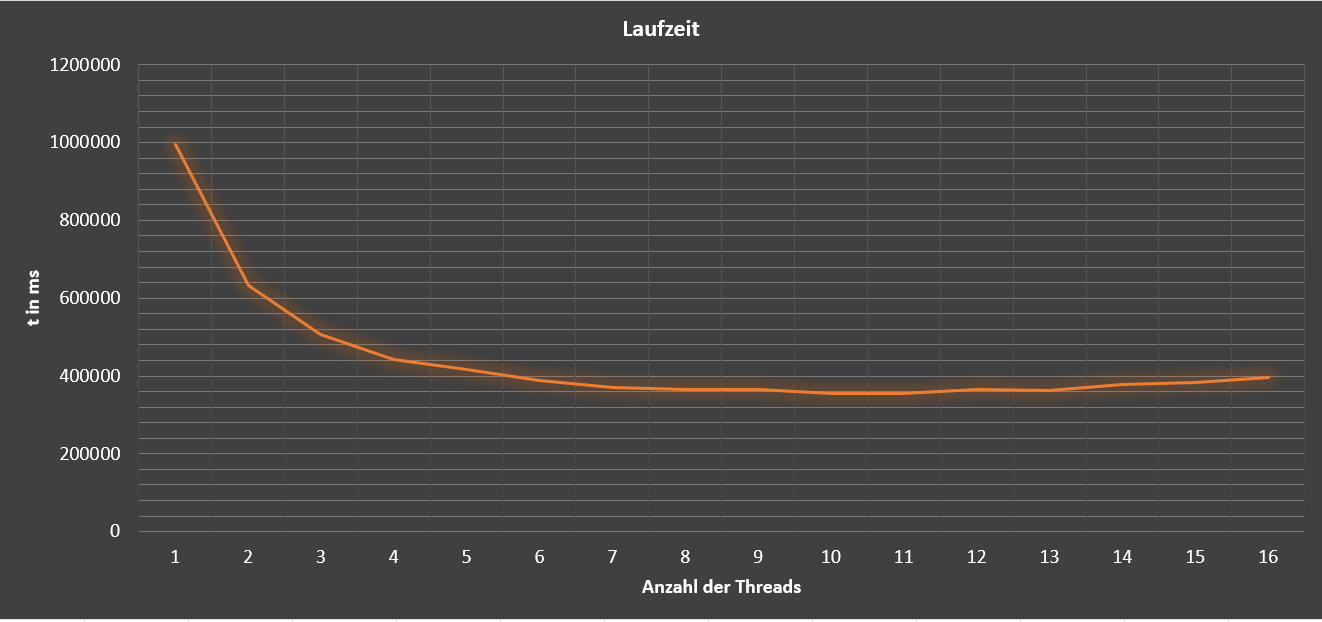
\includegraphics[width=0.8\textwidth]{Base64LaufzeitPic}
	\caption{Laufzeitdiagramm (eigene Abbildung)}
	\label{fig:Base64LaufzeitPic} 
	\end{center}
\end{figure}

Ob die Entwicklung der Laufzeit mit dem Energieverbrauch korreliert, wird anhand der folgen Diagramme diskutiert. In \autoref{fig:Base64LaufzeitPic} wird zunächst die durchschnittliche Leistungsaufnahme des Akkus während der Base64-Kodierung in Abhängigkeit von der Thread-Anzahl dargestellt. Die Leistungswerte für dieses Diagramm  und die dazugehörige \autoref{tab:Base64Leistung} wurden ermittelt, indem das arithmetische Mittel aus den einzelnen Messergebnissen ermittelt wurde. Diese Messergebnisse sind in tabellarischer Form im Anhang zu finden. Der Graph in \autoref{tab:Base64Leistung} zeigt, dass die stärkste Zunahme der durchschnittlichen Leistungsaufnahme bei der Zuschaltung von 2 und 3 Threads zu verzeichnen ist. Auch hierfür ist die initiale Auslastung der beiden Cortex-A73 Rechenkerne verantwortlich. Die höhere Taktrate dieser beiden Kerne verursacht auch eine höhere Leistungsaufnahme verglichen mit den niedrig getakteten Cortex-A53 Kernen. Bis zur Marke von acht Threads ist, wie zu erwarten war, ein relativ konstanter Anstieg im Graphen zu erkennen. Hierbei werden nach und nach die restlichen Cortex-A53 Kerne für die parallele Ausführung hinzugezogen. Erst ab der Verwendung von neun Threads wird der Verlauf unstetig. So fällt die durchschnittliche Leistungsaufnahme bei neun Threads von 3,772 \ac{w} auf 3,662 \ac{w} ab. Danach steig der Graph jedoch wieder bis zum Höchstwert von 3,824 \ac{w} bei 11 Threads. Der kurzzeitige Einbruch bei neun Threads könnte durch die  Ungenauigkeit der Messmethode mittels Battery Historian zustande gekommen sein. Da die Messzeitpunkte für Stromstärke und Spannung in relativ großen Abständen von 30 Sekunden liegen, fallen kurzzeitige Spannungsabfälle und niedrige Entladeströme stärker ins Gewicht der Berechnungen. Davon abgesehen korreliert dieser Verlauf mit dem Diagram aus \autoref{fig:Base64LaufzeitPic}. Die schnellste Ausführung bei 11 Threads zieht demnach die höchste Leistungsaufnahme nach sich. Diese Tatsache stützt außerdem die Begründung der besseren Auslastung der leistungsfähigen Cortex-A73 Rechenkerne bei 11 Threads. Diese erhalten durch den Kontextwechsel mehr Anteile an der Kodierung, was zu höherer Auslastung führt und einen größeren Leistungsaufwand nach sich zieht. \todo{Begründung ab 12 Threads}
% !TeX root = ../my-thesis.tex
% Table generated by Excel2LaTeX from sheet 'Tabelle1'
\begin{table}[htbp]
  \centering
  \caption{durchschnittliche Leistungsaufnahme in Abh\"angigkeit von der Thread Anzahl}
    \begin{tabular}{rrrr}
    \toprule
    \multicolumn{1}{c}{Threads} & \multicolumn{1}{c}{\O U in mV} & \multicolumn{1}{c}{\O I in mA} & \multicolumn{1}{c}{\O P in W} \\
    \midrule
    1     & 4077,382 & 565,944 & 2,306 \\
    \midrule
    2     & 3997,636 & 733,983 & 2,931 \\
    \midrule
    3     & 4029,556 & 860,404 & 3,462 \\
    \midrule
    4     & 4056,719 & 859,178 & 3,479 \\
    \midrule
    5     & 4043,867 & 869,086 & 3,505 \\
    \midrule
    6     & 4028,429 & 900,618 & 3,621 \\
    \midrule
    7     & 4017,545 & 923,407 & 3,705 \\
    \midrule
    8     & 4042,727 & 933,792 & 3,772 \\
    \midrule
    9     & 4063,227 & 901,938 & 3,662 \\
    \midrule
    10    & 4046,045 & 934,489 & 3,775 \\
    \midrule
    11    & 4034,455 & 948,283 & 3,824 \\
    \midrule
    12    & 4074,458 & 856,408 & 3,485 \\
    \midrule
    13    & 4049,000 & 962,385 & 3,486 \\
    \midrule
    14    & 4063,917 & 915,918 & 3,586 \\
    \midrule
    15    & 4021,708 & 926,291 & 3,726 \\
    \midrule
    16    & 4023,542 & 946,001 & 3,806 \\
    \bottomrule
    \end{tabular}%
  \label{tab:Base64Leistung}%
\end{table}%


\begin{figure}[h]
	\begin{center}	 
	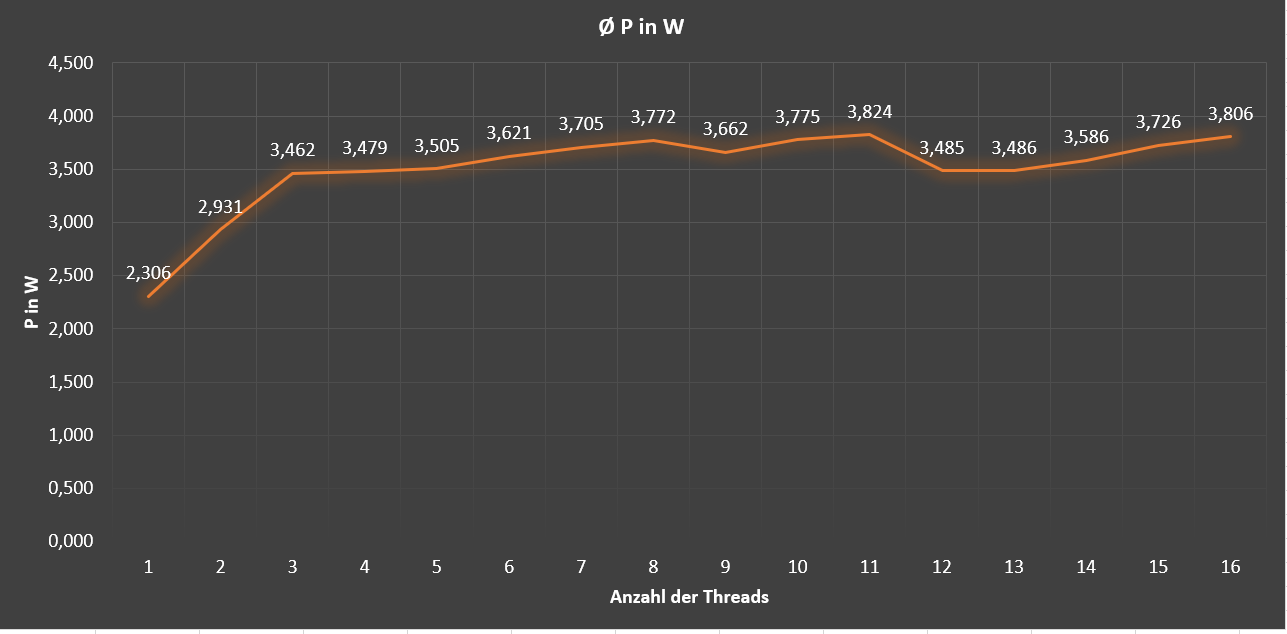
\includegraphics[width=0.8\textwidth]{Base64LeistungPic}
	\caption{durchschnittliche elektrische Leistung in Abhängigkeit von der Thread Anzahl (eigene Abbildung)}
	\label{fig:Base64LeistungPic} 
	\end{center}
\end{figure}

Anhand der bisherigen Betrachtung des Laufzeit- und Leistungsdiagramms konnte festgestellt werden, dass die parallele Ausführung mit steigender Thread-Anzahl bis zur Grenze von 11 Threads zwar schneller verläuft, jedoch mehr Leistungsaufnahme und damit höheren Akkuverbrauch fordert. Nun gilt es zu klären, welcher der beiden Faktoren die Oberhand behält und ob die schnellere Laufzeit trotz der erhöhten Leistungsaufnahme insgesamt zu einer energieeffizienteren Kodierung führt. Zu diesen Zweck wurde für jede Messung die elektrische Leistung über der Zeit abgebildet. Aus dieser Betrachtung ergeben sich für jede Ausführung mit entsprechender Thread-Anzahl Diagrammdarstellungen der Leistung über die Zeit der Ausführung.  In \autoref{fig:Base64LeistungFlächePic} ist exemplarisch ein Leistungsdiagramm der Ausführung mit einem Thread zu sehen. Um eine Bewertung des Energieverbrauchs durchführen zu können, wurde mithilfe dieses Graphen die während der Kodierung verrichtete elektrische Arbeit des Gerätes ermittelt. Hierzu musste die orange unterlegte Fläche unterhalb des Graphen der Leistungskurve bestimmt werden. Da es sich hierbei um unregelmäßige Messewerte handelt, welche sich schlecht auf eine sinnvoll integrierbare Funktionsgleichung abbilden lassen, musste auf das Riemannsche Integral zurückgegriffen werden.\todo{Quelle Mathebuch trapezregel} Hierbei handelt es sich um ein mathematisches Näherungsverfahren zur Bestimmung des Integrals einer reellen Funktion auf einem festgelegten Intervall. Bei diesem Verfahre wird die Fläche unterhalb eines Graphen in beliebig viele Rechtecke aufgeteilt. Die Flächen der Rechtecke werden anschließend aufsummiert und liefern schlussendlich eine Approximation der Gesamtfläche  zwischen dem Graphen und der X-Achse bezüglich des gewählten Intervalls. Um so feingliedriger die Gesamtfläche aufgeteilt wird, um so genauer wird auch die Approximation. Da die Messwertaufnahmen durch Battery Historian in 30 Sekundenabständen durchgeführt werden, ist für die Approximation der elektrischen Arbeit diese Feingliedrigkeit beschränkt. So sind die Rechteckflächen stets 30 Zeiteinheiten breit. Eine so ermittelte Teilfläche, repräsentiert somit die elektrische Arbeit, die während dieser 30 Sekunden verrichtet wurde. Durch die Aufsummierung dieser Werte wird die gesamte elektrische Arbeit während einer Kodierung approximiert. Eine Übersicht der so ermittelten Ergebnisse  für die parallele Base64-Kodierung mit unterschiedlich vielen Threads ist in \autoref{tab:Base64Arbeit} zu finden.

\begin{figure}[H]
	\begin{center}	 
	\includegraphics[width=0.95\textwidth]{Base64LeistungFlächePic}
	\caption{Verlauf der elektrischen Leistung mit einem Thread (eigene Abbildung)}
	\label{fig:Base64LeistungFlächePic} 
	\end{center}
\end{figure}
% !TeX root = ../my-thesis.tex
% Table generated by Excel2LaTeX from sheet 'Tabelle1'
\begin{table}[htbp]
  \centering
  \caption{elektrische Arbeit in Abhängigkeit von der Thread Anzahl}
    \begin{tabular}{rr}
    \toprule
    \multicolumn{1}{c}{Threads} & \multicolumn{1}{c}{W in Ws} \\
    \midrule
    1     & 2330,170 \\
    \midrule
    2     & 1891,658 \\
    \midrule
    3     & 1815,574 \\
    \midrule
    4     & 1594,628 \\
    \midrule
    5     & 1532,691 \\
    \midrule
    6     & 1473,056 \\
    \midrule
    7     & 1347,732 \\
    \midrule
    8     & 1296,977 \\
    \midrule
    9     & 1252,836 \\
    \midrule
    10    & 1290,069 \\
    \midrule
    11    & 1306,284 \\
    \midrule
    12    & 1316,109 \\
    \midrule
    13    & 1322,537 \\
    \midrule
    14    & 1374,502 \\
    \midrule
    15    & 1393,833 \\
    \midrule
    16    & 1409,848 \\
    \bottomrule
    \end{tabular}%
  \label{tab:Base64Arbeit}%
\end{table}%


Der Graph von \autoref{fig:Base64ArbeitPic} zeigt einen kontinuierlichen Abfall der verrichteten Arbeit mit steigender Thread-Anzahl bis zur Marke von neun Threads. Ab 10 Threads steigt der Graph allmählich wieder. Daraus lässt sich ableiten, dass die parallele Durchführung mit neun Threads am energieeffizientesten ist. Allerdings muss an dieser Stelle erwähnt werden, dass durch die verzerrte Leistungsmessung bei der Kodierung mit neun Threads, welche schon in vorherigen Abschnitten erläutert wurde, eine Verschiebung des Wertes der elektrischen Arbeit für neun Threads zustande gekommen sein könnte. Auffällig ist hier der leichte Einbruch des Graphen bei neun Threads, welcher sich ebenfalls in \autoref{fig:Base64LeistungPic} wiederspiegelt. Es könnte daher durchaus diskutiert werden, ob die energieeffizienteste Kodierung doch mit acht Threads erreicht ist. Da der Graph einen stetigen Abfall bis zur Marke von neun Threads zeigt, ist anzunehmen, dass bis zu diesem Punkt der Geschwindigkeitsvorteil und die damit verbundene Verkürzung der Rechenzeit schwerer Wiegt als der Zuwachs der Leistungsaufnahme. Trotz der Tatsache, dass die optimale Laufzeit mit 11 Threads erreicht wurde, steigt der Energieverbrauch ab 10 Threads stetig, da die benötigte Laufzeit für die Kodierung mit neun Threads bis zur Kodierung mit 11 Threads nur noch um 0,9 \% sinkt und die durchschnittliche Leistungsaufnahme im Gegenzug um sieben \% ansteigt. Ab diesem Punkt wiegt der Zuwachs an elektrischer Leistungsaufnahme also stärker als die verringerte Laufzeit und kommt trotz der schnellsten Ausführung zu mehr Stromverbrauch bei 11 Threads. Ab der Marke von 12 Threads ist der stetige Anstieg des Energieverbrauchs einerseits mit der allmählich erhöhten Laufzeit durch das aufwendige Thread-Management und der steigenden beziehungsweise gleichbleibenden Leistungsaufnahme zu begründen.

\begin{figure}[H]
	\begin{center}	 
	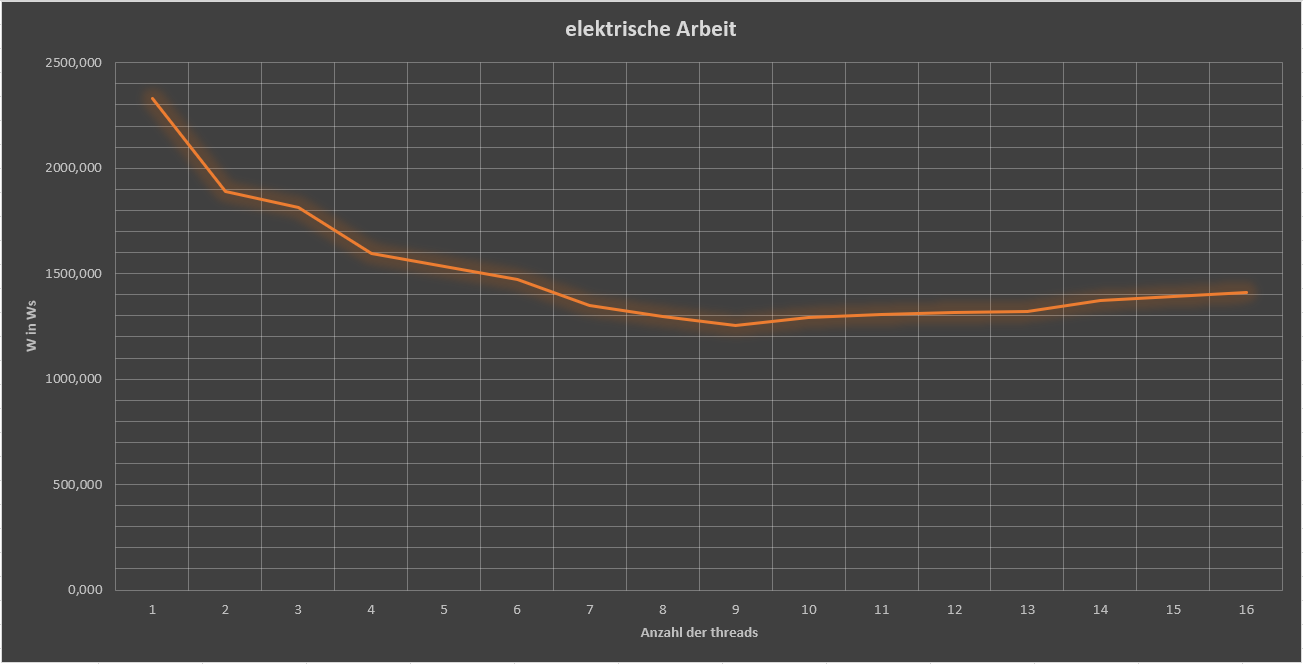
\includegraphics[width=0.95\textwidth]{Base64ArbeitPic}
	\caption{elektrische Arbeit in Abhängigkeit der Thread Anzahl(eigene Abbildung)}
	\label{fig:Base64ArbeitPic} 
	\end{center}
\end{figure}

\section{Gewonnene Erkenntnisse}

Nachdem die Messergebnisse der parallelen Base64-Kodierung im vorherigen Abschnitt dargestellt wurden und mögliche Ursachen für die beobachtete Entwicklung erklärt wurden, folgt in diesem Unterkapitel die Aufzählung der gewonnene Erkenntnisse hinsichtlich der parallelen Ausführung auf mobilen Geräten.

Es konnte bestätigt werden, dass auf einem Gerät mit Mehrkernprozessor die parallele Ausführung von Threads zu einem bestimmten Punkt nicht nur schneller sondern auch Stromsparender wird. Dabei ist allerdings zu beachten, dass die optimale Thread-Anzahl hinsichtlich der Laufzeitoptimierung nicht immer gleich der optimalen Thread-Anzahl hinsichtlich der Energieeffizienz ist. So wurde mit dem hier verwendeten Samsung Galaxy A7 bei der Verwendung von 11 Threads zwar die schnellste Ausführung festgestellt, die energiesparendste Variante war jedoch die Kodierung mit neun Threads. Ein wesentlicher Faktor für diesen Sachverhalt ist der immer kleiner werdende Gewinn an Ausführungsgeschwindigkeit (Speedup) pro zusätzlichen  Thread, bei steigender Leistungsaufnahme. Diese Entwicklung ist sehr gut im Kurvenverlauf von \autoref{fig:Base64LaufzeitPic} zu erkennen. Außerdem wurde festgestellt, dass die Architektur der \ac{cpu} einen erheblichen Einfluss auf die optimale Anzahl von Threads  haben kann. So wurde aufgrund der hier verwendeten Exynos 7885 \ac{soc}-Architektur mit zwei 2,20 \ac{ghz} Kernen und vier 1,60 \ac{ghz} Kernen die erwartete Optimalananzahl von acht Threads, entsprechend der vorhanden acht physischen Rechenkerne, nach oben verschoben. Dies liegt an der besseren Auslastung der zwei stärkeren Kerne durch Kontextwechsel bei der Verwendung von mehr Threads als \ac{cpu}-Kerne. Es ist allerdings zu beachten, dass dies nur im Spezialfall einer Chiparchitektur mit unterschiedlich getakteten Kernen zutrifft. Bei homogenen Architekturen mit ausschließlich gleichartigen Rechenkernen ist zu vermuten, dass die optimale Thread-Anzahl für parallele Berechnungen gleich der Anzahl an vorhanden Prozessorkernen ist. Dies ist hauptsächlich für die Laufzeit der Fall. Hinsichtlich der Energieeffizienz ist zu beachten, dass der prozentuale Gewinn an Laufzeitgeschwindigkeit nicht den Zuwachs an Leistungsaufnahme pro zusätzlichen Thread unterschreitet.